\iffalse
Die Einleitung dient dazu, beim Leser Interesse für die Inhalte 
Praxissemesterberichts zu wecken, die behandelten Probleme aufzuzeigen 
und die zu ihrer Lösung entwickelten Konzepte zu beschreiben.
\fi



\section{Vorangegangene Arbeit}
\label{sec:vorangegangene_arbeit}

\section{Motivation}
\label{sec:motivation}

\iffalse
In der Motivation wird dargestellt, welche Bedeutung die im 
Praxissemester zu entwickelnden Lösungen für das betreuende Unternehmen 
haben. Es wird beispielsweise aufzeigt, in welches Produkt sie eingehen, 
welcher Ablauf verbessert werden soll etc.
\fi

MongoDB hat sich in den letzten Jahren zu einem der wichtigsten Datenbanksysteme entwickelt, da aufgrund immer größerer werdenden Datenmengen die Vorteile von NoSQL-Datenbanken für immer mehr Anwendungen überwiegen.
~\autocite{db-engines:mongodb}
Da MongoDB keine relationale Datenbank ist, können herkömmliche Visualisierungs- und Analysetools, die für SQL entwickelt wurden, nicht verwendet werden.
Für MongoDB gibt es zwar ein paar visualisierungstools wie Beispielsweise MongoDB Charts und MongoDB Compass, die meisten davon visualisieren aber die Daten in der Datenbank, und nicht die Struktur und das Schema der Dokumente in der Datenbank.
~\autocite{knowi:mongo_vis_tools}
Ziel dieses Projekts ist es deshalb, ein Visualisierungstool für MongoDB Datenbanken zu entwickeln, welches die Dokumente der Datenbanken analysiert und auswertet.
Diese Schemas werden dann in Form von verschachtelten Tabellen visualisiert.
Das erleichtert es den Entwicklern der Datenbanken, die Strukturen und Abhängigkeiten in ihren Datenbanken zu verstehen und zu verbessern.


\section{Problemstellung und -abgrenzung}
\label{sec:problemstellung}

Um Datenbanken analysieren zu können, muss es möglich sein, sich mit diesen zu verbinden.
Dies erfordert einerseits eine Nutzeroberfläche, über die der Nutzer die Verbindungsdaten eingeben kann.
Andererseits erfordert dies die Verbindung mit der Datenbank selbst über eine geeignete MongoDB Schnittstelle.
Die Dokumente der Datenbank müssen anschließend in möglichst kurzer Zeit analysiert werden, um aus ihnen Schemas zu extrahieren.
Diese Schemas müssen dann in einem Frontend übersichtlich und visuell ansprechend angezeigt werden.
Dafür werden hauptsächlich 2 Ansichten benötigt:
Einerseits wird eine Übersicht über alle Collections benötigt, in welcher  für jede Collection das meistverwendete Schema angezeigt werden soll.
Andererseits wird für jede Collection eine Detailansicht benötigt, welche alle Schema-Variationen in einer Collection sowie  weitere Details und Daten anzeigt.


Die Problemstellung dient dazu, das zu lösende Problem klar zu 
definieren und abzugrenzen. Der Praktikant soll ein klares Verständnis 
des zu lösenden Problems haben. Insbesondere soll auch verhindert 
werden, dass zu viele Probleme gleichzeitig angegangen werden. Eine 
Negativabgrenzung verhindert, dass beim Leser später nicht erfüllte 
Erwartungen geweckt werden.

\section{Ziel der Arbeit}
\label{sec:ziel}

Mit dem Ziel der Arbeit wird der angestrebte Lösungsumfang festgelegt. An diesem Ziel wird entschieden, ob das Praktikum erfolgreich absolviert wurde oder nicht.

\section{Vorgehen}
\label{sec:vorgehen}

Nachdem mit Problemstellung und Ziel gewissermaßen Anfangs- und Endpunkt 
des Praktikums beschrieben sind, wird hier der zur Erreichung des Ziels 
eingeschlagene Weg vorgestellt. Dazu werden typischerweise die folgenden 
Kapitel und ihr Beitrag zur Erreichung des Ziels der Arbeit kurz 
beschrieben. Die folgenden Kapitel sind ein – möglicher – Aufbau, 
Abweichungen können durchaus notwendig sein. Zur Darstellung des 
Vorgehens ist eine grafische Darstellung sinnvoll, bei der die einzelnen 
Lösungsschritte und ihr Zusammenhang dargestellt werden. Ein Beispiel 
hierfür findet sich in Abbildung \ref{fig:1}.

%\begin{figure}[htbp]
%  \centering
%  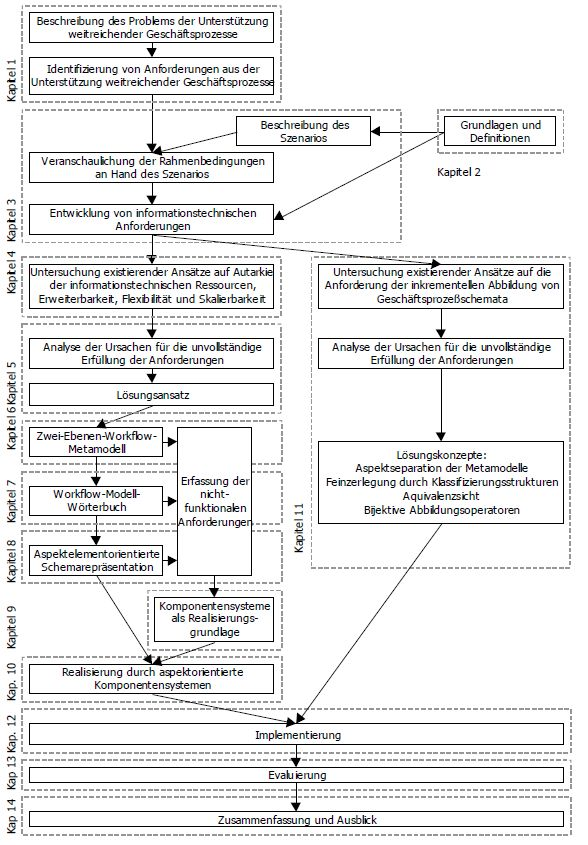
\includegraphics[height=0.9\textheight]{images/ausarbeitung.jpg}
%  \caption{vorgehen nach \autocite{Schmidt:Geschaeftsprozesse}}
%  \label{fig:1}
%\end{figure}

